

%To run this example in the browser through MindQuantum, follow the link:

%\href{https://blog.csdn.net/fisherish/article/details/105115272}{https://blog.csdn.net/fisherish/article/details/105115272}
%\cite{PhysRevLett.131.030402}
View demo code of this section: \democode{05}{5.2}

\subsubsection{Background}

In this section, we present an introduction to the Quantum Approximate Optimization Algorithm (QAOA) and demonstrate its implementation using \MindQuantum. Additionally, we explore advanced applications in Section D, where we apply techniques STA to achieve improved convergence ansatz CD-QAOA \cite{PhysRevResearch.4.013141}.


QAOA is a powerful quantum algorithm designed to address combinatorial optimization problems by harnessing the capabilities of quantum computers. It was first proposed by Farhi et al. in 2014 \cite{farhi2014quantum}, and since then, numerous variants have been developed to overcome the limitations of the original algorithm.

Inspired by the trotterized version of the quantum adiabatic algorithm, QAOA is categorized as a variational quantum algorithm. The conventional QAOA comprises two main components: the quantum part, which involves a parameterized circuit ansatz, and the classical part, responsible for optimizing these parameters. To employ the QAOA algorithm effectively, we define the problem as finding the ground state of a problem Hamiltonian. The ansatz is constructed from two fundamental building blocks, namely the mixer layer and the problem layer:

\begin{equation}
    U(\gamma, \beta) = \prod_{l=1}^p e^{-i\beta_l \hat{H}_{m}}e^{-i\gamma_l\hat{H}{{p}}},
\end{equation}
where $\hat{H}_{{m}} = \sum_i \hat{\sigma}^x_i$ represents the mixer Hamiltonian, where $\hat{\sigma}^x$ corresponds to the Pauli $x$ operator. On the other hand, $\hat{H}_{{p}}$ denotes the problem Hamiltonian.

The quantum state begins from the ground state of $\hat{H}_{\text{mixer}}$, which is $|\psi_0\rangle=|+\rangle^{\otimes n}$. Then, the quantum state for the QAOA ansatz is expressed as:
\begin{equation}
    |\psi_p(\gamma, \beta)\rangle = e^{-i\beta_p\hat{H}_m}e^{-i\gamma_p\hat{H}_p}\cdots e^{-i\beta_1\hat{H}_{m}}e^{-i\gamma_1\hat{H}_{p}}|\psi_0\rangle.
\end{equation}
To determine the cost or objective function, we calculate the expectation value of the problem Hamiltonian $\hat{H}_{\text{prob}}$ with respect to the ansatz state $|\psi_p(\gamma, \beta)\rangle$. This involves performing repeated measurements of the final state in the computational basis:
\begin{equation}
    F_p(\gamma, \beta) =\langle\psi_p(\gamma, \beta)|\hat{H}_{p} |\psi_p(\gamma,\beta)\rangle.
\end{equation}
The primary objective of the QAOA is to find the optimal parameters $(\gamma^*, \beta^*)$ that minimize the expectation value $F_p(\gamma, \beta)$. Achieving this goal involves employing a classical optimization algorithm to iteratively update the parameters $\gamma$ and $\beta$:
\begin{equation}
    (\gamma^*, \beta^*) = \text{arg}\min_{\gamma, \beta} F_p(\gamma, \beta).
\end{equation}

By finding these optimal parameters, QAOA enables quantum computers to efficiently tackle complex optimization challenges, offering a promising avenue for various practical applications.




\subsubsection{Implementation}

For this tutorial, we use QAOA algorithm to handle the Max-Cut problem,  which is an NP-complete problem in graph theory. As shown in figure \ref{5.1_QAOA}, it needs to divide the vertices of a graph into two parts and make the most edges be cut. But when the number of vertices in the graph increases, it is difficult for us to find an effective classical algorithm to solve the Max-Cut problem, because it is very likely that there is no polynomial time algorithm for this type of NP-complete problem.

\begin{figure}[H]
    \centering
    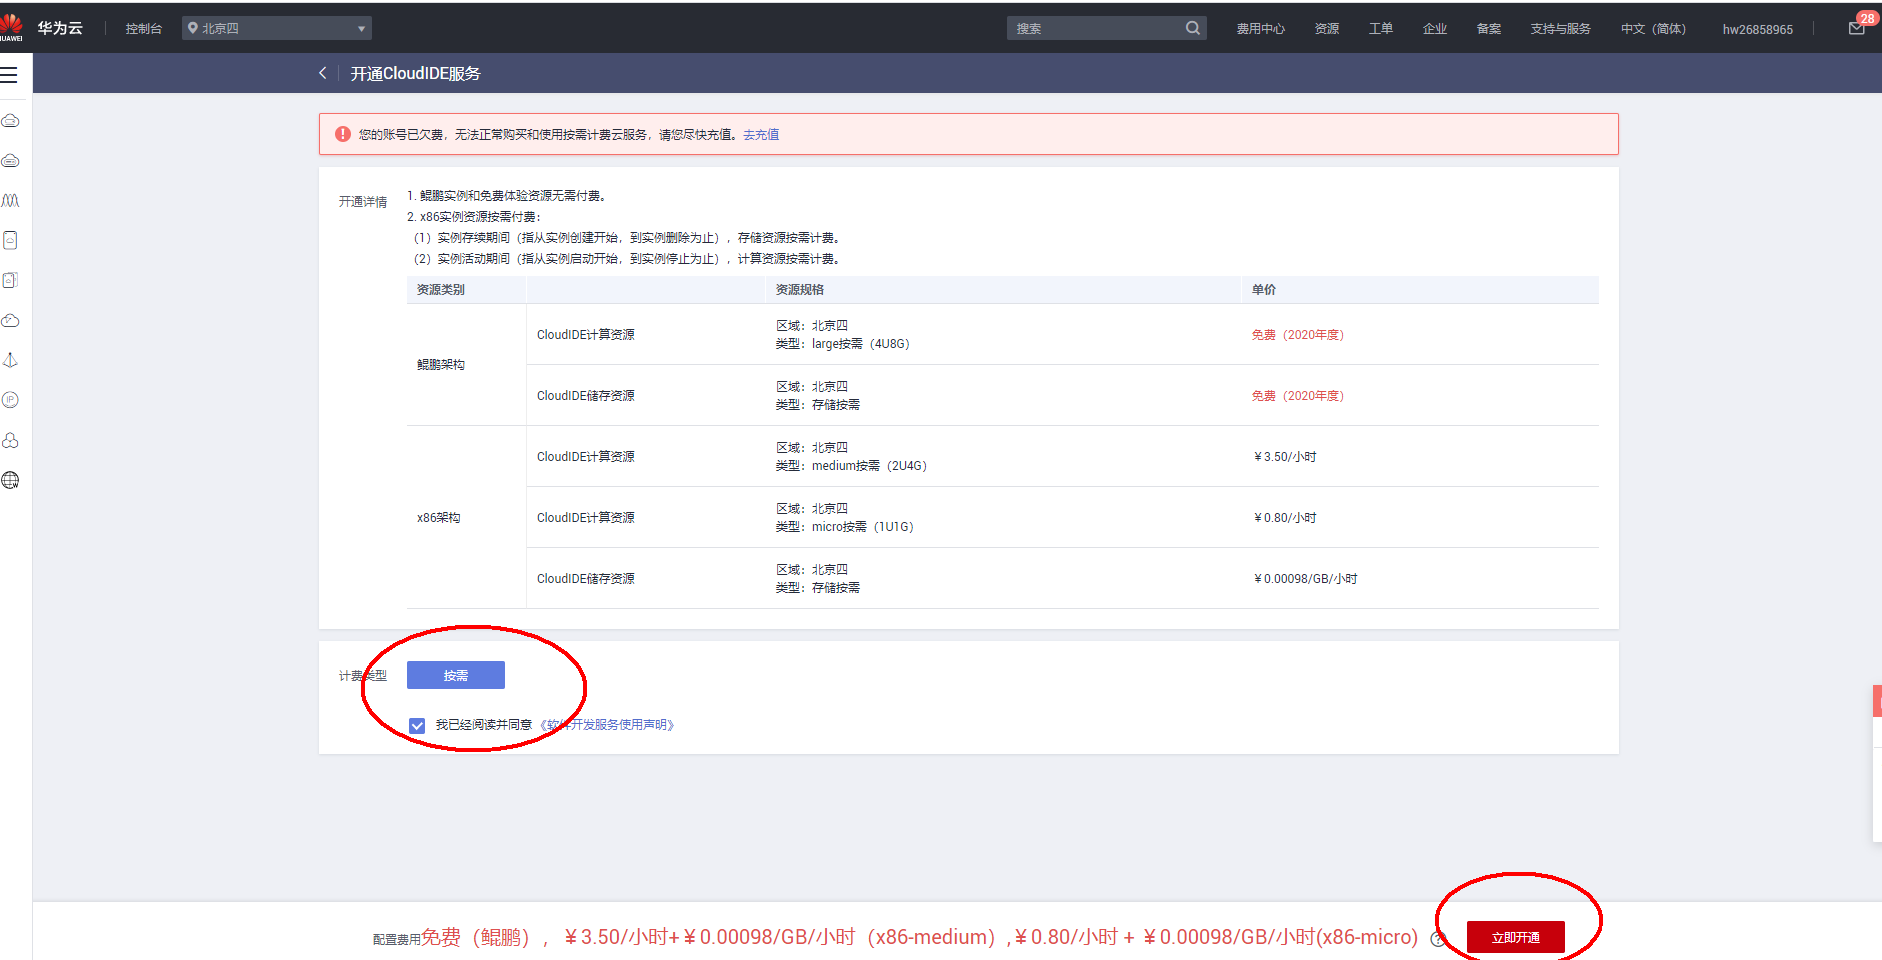
\includegraphics[width=0.49\textwidth]{5.2_figures/5.2_QAOA}
    \caption{Max-cut graph}
    \label{5.1_QAOA}
\end{figure}

Let us first generate a graph structure consisting of five vertices and six edges using NetworkX[cite].
\begin{lstlisting}
g = nx.Graph()
nx.add_path(g, [0,1])
nx.add_path(g, [1,2])
nx.add_path(g, [2,3])
nx.add_path(g, [3,4])
nx.add_path(g, [0,4])
nx.add_path(g, [0,2])
nx.draw(g,with_labels=True, font_weight='bold')
\end{lstlisting}

For QAOA algorithm, first we need to convert the Max-Cut problem into a Hamiltonian, it's ground state energy is solution of the problem. The problem hamitonian of the Max-Cut problem can be built as
\begin{equation}
    \hat{H} = \sum_{i,j\in C}(\hat{Z}_i\hat{Z}_j-1)/2,
\end{equation}
where $C$ is the set of all edges. In the following function, \code{ build\_ham}, the corresponding Hamiltonian can be constructed by inputting the graph.
\begin{lstlisting}
def build_ham(g):
    hc = QubitOperator()
    for i in g.edges:
        hc += QubitOperator(f'Z{i[0]} Z{i[1]}')
    return hc
\end{lstlisting}
Next, construct the QAOA ansatz, in which function \code{build\_hc} and \code{build\_hb} construct the quantum circuit according to the problem Hamiltonian and the mixer Hamiltonian. The ansatz can be directly builded in function \code{build\_ansatz} by inputting the graph.

\begin{lstlisting}
def build_hc(g,para):
    hc = Circuit()
    for i in g.edges:
        hc += ZZ(para).on(i)
    return hc
def build_hb(g, para):
    hc = Circuit()
    for i in g.nodes:
        hc += RX(para).on(i)
    return hc
def build_ansatz(g, p):
    c = Circuit()
    for i in range(p):
        c += build_hc(g,f'g{i}')
        c += build_hb(g,f'b{i}')
    return c
\end{lstlisting}

In this example, p = 4 is selected, indicating that the four-layer QAOA quantum circuit is used.  And \code{init\_state\_circ} is a quantum circuit for preparing a initial state on a uniformly superposed state.
\begin{lstlisting}
p = 4
ham = Hamiltonian(build_ham(g))
ansatz = build_ansatz(g, p)
init_state_circ = UN(H, g.nodes)
\end{lstlisting}

The goal of QAOA is to find the optimal parameters that make the cost function or the expectation of hamitonian $\mathcal{E}=\langle \psi(\gamma, \beta)|\hat{H}|\psi(\gamma, \beta)\rangle$ minimize.
This problem does not require a coding-layer quantum circuit, so we use \MQAnsatzOnlyLayer as a quantum neural network to be trained and the adam as the optimizer.
\begin{lstlisting}
import mindspore as ms
ms.set_context(mode=ms.PYNATIVE_MODE, device_target="CPU")

total_circuit = init_state_circ + ansatz
sim = Simulator('mqvector', total_circuit.n_qubits)
grad_ops = sim.get_expectation_with_grad(ham, total_circuit)
net = MQAnsatzOnlyLayer(grad_ops)
opti = nn.Adam(net.trainable_params(), learning_rate=0.05)
train_net = nn.TrainOneStepCell(net, opti)

for i in range(600):
    if i%10 == 0:
        print("train step:", i, ", cut:", (len(g.edges)-train_net())/2)
\end{lstlisting}
\begin{lstlisting}
train step: 0 ,   cut: [3.0001478]
train step: 10 ,  cut: [4.1718774]
train step: 20 ,  cut: [4.6871986]
train step: 30 ,  cut: [4.7258005]
train step: 40 ,  cut: [4.804503]
train step: 50 ,  cut: [4.8477592]
train step: 60 ,  cut: [4.8705964]
train step: 70 ,  cut: [4.9060946]
train step: 80 ,  cut: [4.933446]
train step: 90 ,  cut: [4.9356637]
train step: 100 , cut: [4.938308]
train step: 110 , cut: [4.9390197]
train step: 120 , cut: [4.939068]
train step: 130 , cut: [4.9392157]
train step: 140 , cut: [4.939249]
train step: 150 , cut: [4.939247]
train step: 160 , cut: [4.939255]
train step: 170 , cut: [4.939257]
train step: 180 , cut: [4.939257]
train step: 190 , cut: [4.939257]
\end{lstlisting}

According to the above training results, we found that the number of edge cuts corresponding to the ground state energy of the Hamiltonian of this problem approaches 5.

In \MindQuantum, we can directly import the function \MaxCutAnsatz to build ansatz for the maxcut problem.
\begin{lstlisting}
import numpy as np
from mindquantum.algorithm.nisq import MaxCutAnsatz
graph = [(0, 1), (1, 2), (0, 2)]
p = 1 # layer
maxcut = MaxCutAnsatz(graph, p)
maxcut.circuit.svg()
\end{lstlisting}
\begin{figure}[H]
    \centering
    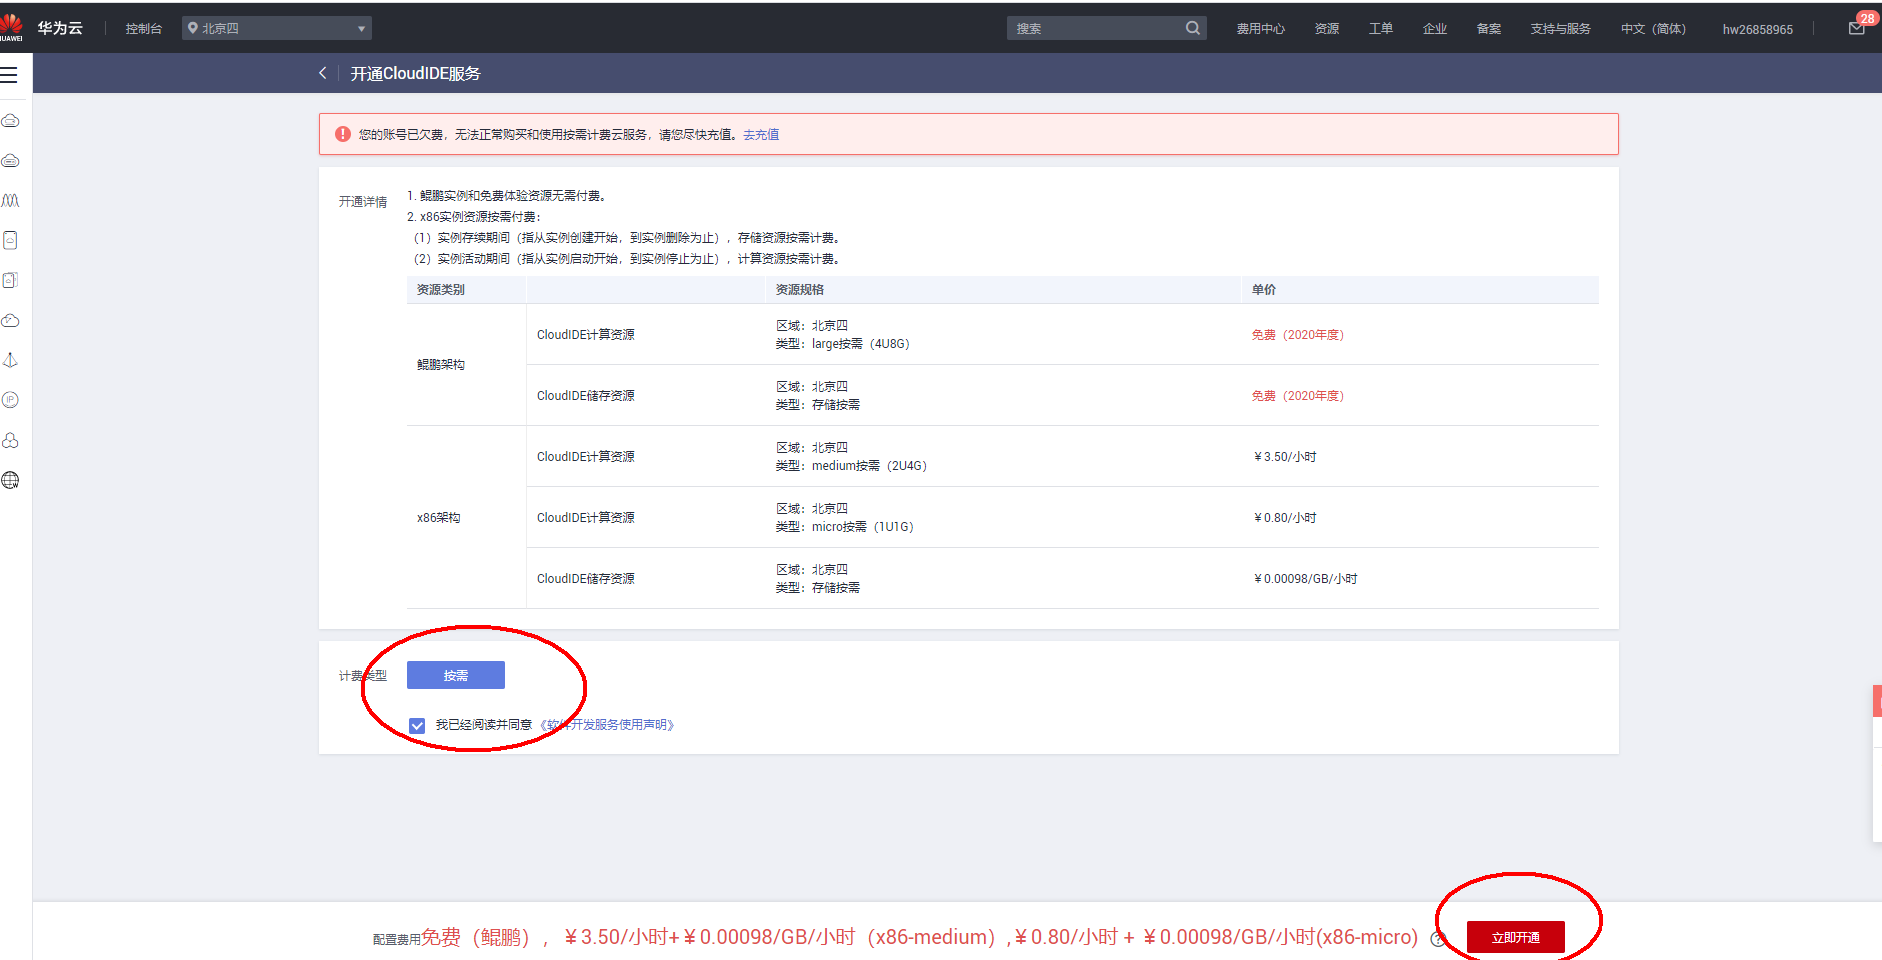
\includegraphics[width=0.49\textwidth]{5.2_figures/5.2_QAOA_ansatze}
    \caption{Max-cut problem Ansatze}
    \label{5.1_QAOA_ansatz}
\end{figure}
At the same time, the Hamiltonian can also be obtained
\begin{lstlisting}
print(maxcut.hamiltonian)
\end{lstlisting}
\begin{lstlisting}
3/2 [] +
-1/2 [Z0 Z1] +
-1/2 [Z1 Z2] +
-1/2 [Z0 Z2]
\end{lstlisting}
The cutting scheme of the MaxCut problem and the number of cutting edges of the cutting scheme can be obtained through the function $get\_partition$ and $get\_cut\_value$. The cutting scheme is a list array consisting of two list arrays, and each list array contains the cut nodes.
\begin{lstlisting}
partitions = maxcut.get_partition(5, np.array([4, 1]))
for i in partitions:
    print(f'partition: left: {i[0]}, right: {i[1]}, cut value: {maxcut.get_cut_value(i)}')
\end{lstlisting}
\begin{lstlisting}
partition: left: [0, 2],   right: [1], cut value: 2
partition: left: [1, 2],   right: [0], cut value: 2
partition: left: [1],   right: [0, 2], cut value: 2
partition: left: [0, 1, 2], right: [], cut value: 0
partition: left: [], right: [0, 1, 2], cut value: 0
\end{lstlisting}










